% !TEX root = ../main.tex
% =====================================================================
% APPENDIX B -- ADDITIONAL RESULTS
%
% Rule: if removing an item would break an argument in Section 5 or 6,
% it belongs there. Everything else that still supports the story is
% here, each item with one table or figure and a short comment.
% =====================================================================

\section{Additional Results}
\label{app:additional}

% ---------------------------------------------------------------------
\subsection{Full leaderboard}
\label{app:leaderboard}

\Cref{tab:web_main} keeps only the headline models and the baselines. The table below lists every
encoder $\times$ pooling head combination trained, ranked by \webtraffic{} accuracy, together with
the configuration identifier of each one, so that any model named in this report can be looked up.

% The generated table has 13 columns and sets its own \small, which is ~30% too wide for this
% page. Locally turning \small into \tiny inside this group shrinks it to fit, without editing the
% generated file (which python main.py paper would overwrite anyway).
% No \clearpage here any more: it was needed when the appendix floats were forced with
% [H], but every float is [htbp] now, so LaTeX can give this table a float page of its
% own. The \clearpage was costing an almost empty page just before it.
{\let\small\tiny
 \setlength{\tabcolsep}{0.75pt}
 \begin{table}[t]
\centering
\small
\caption{Complete leaderboard: all 72 evaluated models, ranked by WebTraffic accuracy. The Model column is the configuration identifier under configs/models/, so any model named in the report can be looked up here. Encoder and pooling names are prefixed sea\_ for components introduced in this work and mil\_ for components reused unchanged from MILLET. A dash marks a model screened on WebTraffic only.}
\label{tab:full_leaderboard}
\begin{tabular}{lrrrrrrrrrrrr}
\toprule
\# & Model & Encoder & Pooling & Origin & Acc. & AOPCR & NDCG & Loss & \#DS & UCR-85 Acc. & Params & Size (MB) \\
\midrule
1 & seanet\_gated\_mean\_topk & sea\_mstcn\_sep\_gated & sea\_topk\_conjunctive & ours & 0.955 & 2.23 & 0.750 & 0.254 & 85 & 0.8083 & 61,740 & 1.50 \\
2 & seanet\_conjunctive & sea\_mstcn\_sep & mil\_conjunctive & half-ours & 0.954 & 1.50 & 0.698 & 0.262 & 85 & 0.8238 & 269,083 & 3.54 \\
3 & seanet\_gated\_max\_topk & sea\_mstcn\_sep\_gated & sea\_topk\_conjunctive & ours & 0.952 & 2.27 & 0.719 & 0.308 & 85 & 0.8108 & 61,740 & 1.50 \\
4 & seanet\_topk\_nofocus & sea\_mstcn\_sep\_bottleneck & sea\_topk\_conjunctive & ours & 0.950 & 2.30 & 0.765 & 0.263 & 0 & -- & 41,324 & 1.43 \\
5 & seanet\_spiketrend\_topk & sea\_mstcn\_sep\_spiketrend & sea\_topk\_conjunctive & ours & 0.950 & 2.32 & 0.756 & 0.288 & 85 & 0.8089 & 67,020 & 1.52 \\
6 & seanet\_inputgate\_mschan & sea\_multiscale\_channels & sea\_topk\_conjunctive & ours & 0.948 & 2.32 & 0.757 & 0.318 & 0 & -- & 69,768 & 1.54 \\
7 & seanet\_gated\_mschan & sea\_multiscale\_channels & sea\_topk\_conjunctive & ours & 0.948 & 2.22 & 0.717 & 0.289 & 0 & -- & 67,592 & 1.53 \\
8 & seanet\_bottleneck\_topk & sea\_mstcn\_sep\_bottleneck & sea\_topk\_conjunctive & ours & 0.947 & 2.62 & 0.772 & 0.282 & 85 & 0.8097 & 41,324 & 1.43 \\
9 & seanet\_recon\_adaptive & sea\_mstcn\_sep\_recon & sea\_adaptive\_classwise & ours & 0.946 & 2.60 & 0.768 & 0.296 & 85 & 0.8140 & 62,935 & 1.51 \\
10 & seanet\_inputgate\_topk & sea\_mstcn\_sep\_inputgate & sea\_topk\_conjunctive & ours & 0.946 & 2.80 & 0.748 & 0.261 & 85 & 0.8131 & 58,092 & 1.49 \\
11 & seanet\_classwise & sea\_mstcn\_sep & sea\_classwise\_conjunctive & ours & 0.946 & 1.72 & 0.686 & 0.292 & 85 & 0.8292 & 269,164 & 3.54 \\
12 & seanet\_gated\_max & sea\_mstcn\_sep\_gated & sea\_classwise\_conjunctive & ours & 0.944 & 1.89 & 0.592 & 0.306 & 85 & 0.8237 & 61,740 & 1.50 \\
13 & seanet\_gated\_last\_topk & sea\_mstcn\_sep\_gated & sea\_topk\_conjunctive & ours & 0.942 & 2.31 & 0.748 & 0.328 & 85 & 0.8015 & 61,740 & 1.50 \\
14 & seanet & sea\_mstcn\_sep & mil\_additive & half-ours & 0.942 & 1.58 & 0.729 & 0.260 & 85 & 0.8298 & 269,083 & 3.54 \\
15 & seanet\_gated\_last & sea\_mstcn\_sep\_gated & sea\_classwise\_conjunctive & ours & 0.942 & 2.52 & 0.742 & 0.327 & 85 & 0.7888 & 61,740 & 1.50 \\
16 & seanet\_recon\_topk & sea\_mstcn\_sep\_recon & sea\_topk\_conjunctive & ours & 0.940 & 2.51 & 0.698 & 0.321 & 85 & 0.8063 & 62,925 & 1.51 \\
17 & seanet\_topk\_k025 & sea\_mstcn\_sep\_bottleneck & sea\_topk\_conjunctive & ours & 0.940 & 2.65 & 0.733 & 0.277 & 0 & -- & 41,324 & 1.43 \\
18 & seanet\_bottleneck\_softmax & sea\_mstcn\_sep\_bottleneck & sea\_softmax\_conjunctive & ours & 0.940 & 1.68 & 0.740 & 0.345 & 85 & 0.8106 & 41,325 & 1.43 \\
19 & seanet\_gated\_last\_adaptive & sea\_mstcn\_sep\_gated & sea\_adaptive\_classwise & ours & 0.938 & 2.39 & 0.793 & 0.289 & 85 & 0.8029 & 61,750 & 1.50 \\
20 & seanet\_spiketrend\_adaptive & sea\_mstcn\_sep\_spiketrend & sea\_adaptive\_classwise & ours & 0.934 & 1.91 & 0.747 & 0.301 & 85 & 0.8010 & 67,030 & 1.53 \\
21 & seanet\_recon\_softmax & sea\_mstcn\_sep\_recon & sea\_softmax\_conjunctive & ours & 0.932 & 1.64 & 0.723 & 0.341 & 0 & -- & 62,926 & 1.51 \\
22 & seanet\_slim\_topk & sea\_mstcn\_sep & sea\_topk\_conjunctive & ours & 0.932 & 2.69 & 0.778 & 0.306 & 85 & 0.8093 & 57,580 & 1.48 \\
23 & seanet\_bottleneck\_gatedattn & sea\_mstcn\_sep\_bottleneck & sea\_gated\_attention & ours & 0.930 & 2.23 & 0.741 & 0.313 & 85 & 0.8146 & 41,844 & 1.43 \\
24 & seanet\_spiketrend\_gatedattn & sea\_mstcn\_sep\_spiketrend & sea\_gated\_attention & ours & 0.930 & 1.59 & 0.721 & 0.350 & 85 & 0.8039 & 67,540 & 1.53 \\
25 & seanet\_gated & sea\_mstcn\_sep\_gated & sea\_classwise\_conjunctive & ours & 0.930 & 2.41 & 0.637 & 0.359 & 85 & 0.7900 & 61,740 & 1.50 \\
26 & seanet\_slim\_adaptive & sea\_mstcn\_sep & sea\_adaptive\_classwise & ours & 0.930 & 2.45 & 0.793 & 0.336 & 0 & -- & 57,590 & 1.49 \\
27 & seanet\_bottleneck\_mschan & sea\_multiscale\_channels & sea\_topk\_conjunctive & ours & 0.926 & 2.24 & 0.777 & 0.357 & 0 & -- & 47,176 & 1.45 \\
28 & seanet\_bottleneck\_mschan\_lean & sea\_multiscale\_channels & sea\_topk\_conjunctive & ours & 0.924 & 2.76 & 0.735 & 0.389 & 0 & -- & 43,576 & 1.44 \\
29 & seanet\_gated\_last\_softmax & sea\_mstcn\_sep\_gated & sea\_softmax\_conjunctive & ours & 0.920 & 1.99 & 0.738 & 0.381 & 0 & -- & 61,741 & 1.50 \\
30 & millet\_paper & mil\_inceptiontime & mil\_conjunctive & millet & 0.920 & 13.27 & 0.661 & 0.371 & 84 & 0.8434 & 423,707 & 4.11 \\
31 & seanet\_acp & sea\_mstcn\_sep & sea\_adaptive\_classwise & ours & 0.918 & 1.61 & 0.619 & 0.360 & 85 & 0.8134 & 269,174 & 3.54 \\
32 & seanet\_gated\_last\_gatedattn & sea\_mstcn\_sep\_gated & sea\_gated\_attention & ours & 0.918 & 1.35 & 0.757 & 0.365 & 85 & 0.8048 & 62,260 & 1.50 \\
33 & seanet\_slim & sea\_mstcn\_sep & sea\_classwise\_conjunctive & ours & 0.916 & 2.48 & 0.719 & 0.383 & 0 & -- & 57,580 & 1.48 \\
34 & seanet\_gated\_max\_softmax & sea\_mstcn\_sep\_gated & sea\_softmax\_conjunctive & ours & 0.914 & 1.88 & 0.776 & 0.372 & 0 & -- & 61,741 & 1.50 \\
35 & seanet\_inputgate & sea\_mstcn\_sep\_inputgate & sea\_classwise\_conjunctive & ours & 0.914 & 2.48 & 0.715 & 0.398 & 0 & -- & 58,092 & 1.49 \\
36 & seanet\_gated\_mean\_softmax & sea\_mstcn\_sep\_gated & sea\_softmax\_conjunctive & ours & 0.912 & 2.09 & 0.765 & 0.368 & 0 & -- & 61,741 & 1.50 \\
37 & seanet\_recon & sea\_mstcn\_sep\_recon & sea\_classwise\_conjunctive & ours & 0.910 & 2.50 & 0.680 & 0.417 & 0 & -- & 62,925 & 1.51 \\
38 & seanet\_topk\_k100 & sea\_mstcn\_sep\_bottleneck & sea\_topk\_conjunctive & ours & 0.908 & 2.44 & 0.722 & 0.395 & 0 & -- & 41,324 & 1.43 \\
39 & seanet\_gated\_max\_adaptive & sea\_mstcn\_sep\_gated & sea\_adaptive\_classwise & ours & 0.906 & 2.07 & 0.729 & 0.444 & 0 & -- & 61,750 & 1.50 \\
40 & seanet\_inputgate\_adaptive & sea\_mstcn\_sep\_inputgate & sea\_adaptive\_classwise & ours & 0.905 & 2.65 & 0.732 & 0.390 & 85 & 0.8153 & 58,102 & 1.49 \\
41 & seanet\_spiketrend & sea\_mstcn\_sep\_spiketrend & sea\_classwise\_conjunctive & ours & 0.904 & 2.15 & 0.699 & 0.395 & 0 & -- & 67,020 & 1.52 \\
42 & seanet\_bottleneck & sea\_mstcn\_sep\_bottleneck & sea\_classwise\_conjunctive & ours & 0.902 & 2.57 & 0.733 & 0.395 & 0 & -- & 41,324 & 1.43 \\
43 & seanet\_gated\_mean & sea\_mstcn\_sep\_gated & sea\_classwise\_conjunctive & ours & 0.902 & 2.49 & 0.714 & 0.393 & 0 & -- & 61,740 & 1.50 \\
44 & seanet\_inputgate\_softmax & sea\_mstcn\_sep\_inputgate & sea\_softmax\_conjunctive & ours & 0.894 & 1.64 & 0.696 & 0.454 & 0 & -- & 58,093 & 1.49 \\
45 & seanet\_slim\_gatedattn & sea\_mstcn\_sep & sea\_gated\_attention & ours & 0.894 & 2.30 & 0.714 & 0.403 & 0 & -- & 58,100 & 1.49 \\
46 & seanet\_recon\_attnmax & sea\_mstcn\_sep\_recon & sea\_attention\_max & ours & 0.892 & 2.32 & 0.725 & 0.499 & 0 & -- & 62,935 & 1.51 \\
47 & seanet\_slim\_softmax & sea\_mstcn\_sep & sea\_softmax\_conjunctive & ours & 0.890 & 1.83 & 0.705 & 0.419 & 0 & -- & 57,581 & 1.49 \\
48 & seanet\_slim\_gatedattn & sea\_mstcn\_sep\_gated & mil\_attention & half-ours & 0.888 & 2.40 & 0.710 & 0.426 & 0 & -- & 58,100 & 1.49 \\
49 & seanet\_topk\_k005 & sea\_mstcn\_sep\_bottleneck & sea\_topk\_conjunctive & ours & 0.888 & 2.29 & 0.715 & 0.401 & 0 & -- & 41,324 & 1.43 \\
50 & millet & mil\_inceptiontime & mil\_conjunctive & millet & 0.887 & 2.57 & 0.677 & 0.507 & 84 & 0.8274 & 423,707 & 4.11 \\
51 & seanet\_gated\_max\_attnmax & sea\_mstcn\_sep\_gated & sea\_attention\_max & ours & 0.886 & 1.12 & 0.575 & 0.588 & 0 & -- & 61,750 & 1.50 \\
52 & seanet\_topk\_k050 & sea\_mstcn\_sep\_bottleneck & sea\_topk\_conjunctive & ours & 0.882 & 3.11 & 0.732 & 0.418 & 0 & -- & 41,324 & 1.43 \\
53 & seanet\_softmax & sea\_mstcn\_sep & sea\_softmax\_conjunctive & ours & 0.880 & 1.02 & 0.605 & 0.455 & 85 & 0.8131 & 269,165 & 3.54 \\
54 & seanet\_spiketrend\_softmax & sea\_mstcn\_sep\_spiketrend & sea\_softmax\_conjunctive & ours & 0.878 & 1.43 & 0.665 & 0.488 & 0 & -- & 67,021 & 1.53 \\
55 & seanet\_bottleneck\_adaptive & sea\_mstcn\_sep\_bottleneck & sea\_adaptive\_classwise & ours & 0.868 & 1.97 & 0.680 & 0.559 & 6 & 0.7772 & 41,334 & 1.43 \\
56 & seanet\_slim\_dualstream & sea\_mstcn\_sep & sea\_dualstream\_conjunctive & ours & 0.860 & 2.40 & 0.745 & 0.498 & 0 & -- & 58,101 & 1.49 \\
57 & seanet\_gated\_mean\_adaptive & sea\_mstcn\_sep\_gated & sea\_adaptive\_classwise & ours & 0.860 & 2.24 & 0.731 & 0.549 & 0 & -- & 61,750 & 1.50 \\
58 & seanet\_inputgate\_attnmax & sea\_mstcn\_sep\_inputgate & sea\_attention\_max & ours & 0.858 & 2.15 & 0.700 & 0.625 & 0 & -- & 58,102 & 1.49 \\
59 & seanet\_spiketrend\_attnmax & sea\_mstcn\_sep\_spiketrend & sea\_attention\_max & ours & 0.854 & 1.65 & 0.644 & 0.637 & 0 & -- & 67,030 & 1.53 \\
60 & seanet\_gated\_last\_attnmax & sea\_mstcn\_sep\_gated & sea\_attention\_max & ours & 0.854 & 1.78 & 0.668 & 0.598 & 0 & -- & 61,750 & 1.50 \\
61 & seanet\_bottleneck\_shallow & sea\_mstcn\_sep\_bottleneck & sea\_topk\_conjunctive & ours & 0.846 & 2.82 & 0.624 & 0.579 & 0 & -- & 21,548 & 1.33 \\
62 & seanet\_gated\_mean\_attnmax & sea\_mstcn\_sep\_gated & sea\_attention\_max & ours & 0.832 & 1.67 & 0.704 & 0.665 & 0 & -- & 61,750 & 1.50 \\
63 & seanet\_gated\_pyramid & sea\_multiscale\_pyramid & sea\_topk\_conjunctive & ours & 0.832 & 0.98 & 0.591 & 0.602 & 0 & -- & 62,781 & 1.52 \\
64 & seanet\_bottleneck\_dualstream & sea\_mstcn\_sep\_bottleneck & sea\_dualstream\_conjunctive & ours & 0.824 & 2.04 & 0.652 & 0.638 & 0 & -- & 41,845 & 1.43 \\
65 & seanet\_bottleneck\_attnmax & sea\_mstcn\_sep\_bottleneck & sea\_attention\_max & ours & 0.816 & 1.74 & 0.610 & 0.732 & 0 & -- & 41,334 & 1.43 \\
66 & seanet\_bottleneck\_pyramid & sea\_multiscale\_pyramid & sea\_topk\_conjunctive & ours & 0.786 & 1.03 & 0.569 & 0.759 & 0 & -- & 42,365 & 1.44 \\
67 & resnet & mil\_resnet & mil\_conjunctive & millet & 0.772 & 2.95 & 0.554 & 0.824 & 85 & 0.8146 & 506,331 & 4.42 \\
68 & fcn & mil\_fcn & mil\_conjunctive & millet & 0.742 & 3.83 & 0.533 & 0.910 & 85 & 0.8141 & 267,035 & 3.47 \\
69 & seanet\_gated\_last\_dualstream & sea\_mstcn\_sep\_gated & sea\_dualstream\_conjunctive & ours & 0.736 & 1.95 & 0.637 & 0.804 & 0 & -- & 62,261 & 1.50 \\
70 & seanet\_slim\_attnmax & sea\_mstcn\_sep & sea\_attention\_max & ours & 0.714 & 1.63 & 0.532 & 0.855 & 0 & -- & 57,590 & 1.49 \\
71 & seanet\_bottleneck\_mschan\_pyramid & sea\_multiscale\_pyramid & sea\_topk\_conjunctive & ours & 0.696 & 2.17 & 0.653 & 0.992 & 0 & -- & 28,441 & 1.37 \\
72 & seanet\_spiketrend\_dualstream & sea\_mstcn\_sep\_spiketrend & sea\_dualstream\_conjunctive & ours & 0.556 & 1.64 & 0.510 & 1.260 & 0 & -- & 67,541 & 1.53 \\
\bottomrule
\end{tabular}
\end{table}
}

The \#DS column reports how many \ucr{} datasets each model completed: a dash or a small number
means the model was screened on \webtraffic{} only, and the 28 models that completed the archive are
the ones ranked in \Cref{tab:ucr_accuracy}. The \texttt{millet\_paper} row is \millet{}'s own long
configuration run on this pipeline; its AOPCR of 13.27 is the direct evidence that AOPCR is
unnormalised (\Cref{sec:disc:reading}).

% ---------------------------------------------------------------------
\subsection{Model cost}
\label{app:cost}

\Cref{sec:res:web} states the headline of this table; the measurements behind it are given here.

\begin{table}[htbp]
\caption{Cost of each model, measured on the real \webtraffic{} input (series of length 1{,}008,
10 classes) on one GPU. ``One prediction'' is the time to classify a single series. ``Training
time'' is the wall-clock time to convergence including early stopping, over the 3 \webtraffic{}
seeds.}
\label{tab:cost}
\begin{center}
\footnotesize
\setlength{\tabcolsep}{5pt}
\begin{tabular}{lrrrr}
\toprule
\textbf{Model} & \textbf{Params} & \textbf{Size (MB)} &
\textbf{1 prediction (ms)} & \textbf{Train (s)} \\
\midrule
\mbot{}                   & \textbf{41{,}324}  & \textbf{1.43} & 0.131 & $117.3\pm14.0$ \\
\minp{}                   & 58{,}102  & 1.49 & 0.128 & $105.8\pm37.2$ \\
\mgat{}                   & 61{,}740  & 1.50 & 0.128 & $91.3\pm25.9$ \\
\millet{}, re-trained here & 423{,}707 & 4.11 & 0.203 & $50.4\pm9.5$ \\
ResNet $+$ conjunctive     & 506{,}331 & 4.42 & 0.139 & 38.1 \\
FCN $+$ conjunctive        & 267{,}035 & 3.47 & \textbf{0.068} & 20.8 \\
\bottomrule
\end{tabular}
\end{center}
\end{table}
% Params / Size / inference time: results/SEA_NET/profile.csv, re-measured 2026-08-09 at
% length 1008, 10 classes, batch 32. The FLOPs column of that file is deliberately not shown here;
% the same information is carried by parameters + prediction time.
% Train time: the WebTraffic rows of each model's results.csv, mean +- std over seeds 0/1/2.

The last column is the counterweight: the \seanet{} models take two to three times longer to train
than the baseline, on every seed. Training time here is wall-clock time until early stopping fires,
so it measures how many epochs a model needed rather than the cost of one epoch, and the baseline
stops improving sooner. Prediction time is the fair per-step comparison, and there \seanet{} is
faster.

% ---------------------------------------------------------------------
\subsection{Ablation studies}
\label{app:ablations}

These ablations answer three questions: does the gain come from the encoder, from the pooling head
or from their combination; how much does $\kappa$ matter; and what does the attention entropy term
buy?

% MUST NOT be [H]: this figure is ~340 pt tall plus its caption and lands right after the
% full-page leaderboard table, so it needs to be free to move.
\begin{figure}[htbp]
  \centering
  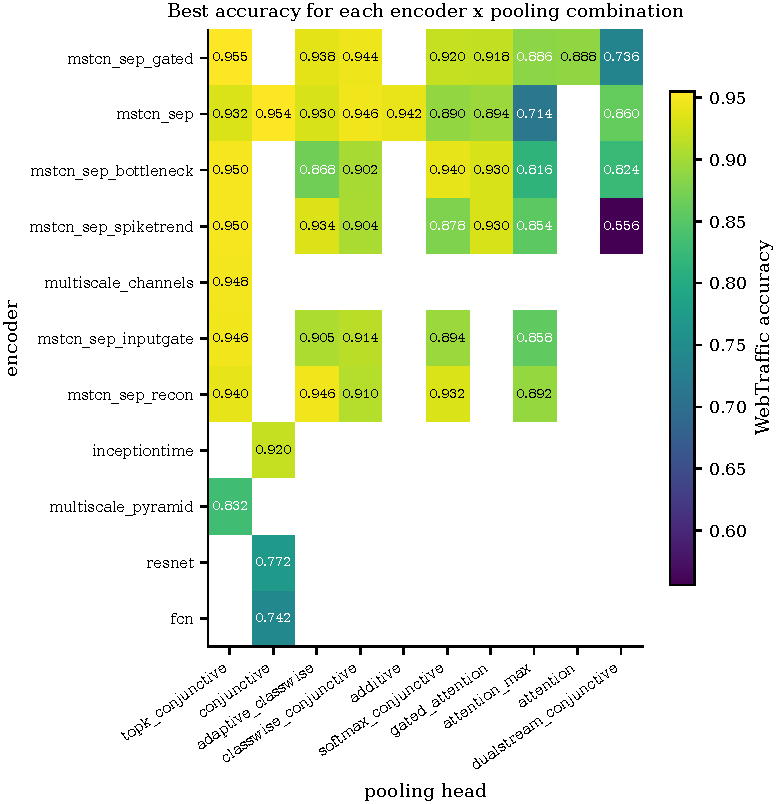
\includegraphics[width=0.66\linewidth]{results/paper_figures/02_ablation/ablation_encoder_pooling_grid}
  \caption{Best \webtraffic{} accuracy for every encoder (rows) and every pooling head (columns).
  One cell is what that pair achieved; blank cells are pairs that were never trained. Rows and
  columns are sorted by their best value, so the strongest components appear towards the top left.}
  \label{fig:ablation_grid}
\end{figure}

\paragraph{A. Effect of the pooling head, averaged over encoders.}
Averaged over every encoder it was paired with, the pooling head alone moves \webtraffic{} accuracy
by almost 18 points.

\begin{table}[htbp]
\caption{\webtraffic{} accuracy, AOPCR and NDCG@$n$ averaged over every encoder each pooling head
was paired with; $n$ is the number of pairings averaged. The three \millet{} heads at the bottom are
shown for reference, but two of them were only ever paired with InceptionTime, so their $n=1$ rows
are not comparable with a head averaged over ten pairings.}
\label{tab:ablation_pooling}
\begin{center}
\footnotesize
\begin{tabular}{lcccr}
\toprule
\textbf{Pooling head} & \textbf{Mean accuracy} & \textbf{Mean AOPCR} & \textbf{Mean NDCG@$n$} & \textbf{$n$} \\
\midrule
Class-wise conjunctive (\Cref{sec:pool:classwise})  & 0.921 & 2.322 & 0.692 & 10 \\
Per-class gated attention (\Cref{sec:pool:gated})   & 0.918 & 1.869 & 0.733 & 4 \\
Adaptive class-wise (\Cref{sec:pool:adaptive})      & 0.912 & 2.210 & 0.732 & 9 \\
Softmax conjunctive (\Cref{sec:pool:softmax})       & 0.907 & 1.690 & 0.712 & 9 \\
Top-$k$ conjunctive (\Cref{sec:pool:topk})          & 0.904 & 2.267 & 0.712 & 16 \\
Attention-max (\Cref{sec:pool:attnmax})             & 0.838 & 1.758 & 0.645 & 8 \\
Dual-stream conjunctive (\Cref{sec:pool:dsmil})     & 0.744 & 2.007 & 0.636 & 4 \\
\midrule
\millet{} additive \citep{early2024millet}          & 0.942 & 1.579 & 0.729 & 1 \\
\millet{} attention \citep{early2024millet}         & 0.888 & 2.403 & 0.710 & 1 \\
\millet{} conjunctive \citep{early2024millet}       & 0.839 & 2.712 & 0.616 & 4 \\
\bottomrule
\end{tabular}
\end{center}
\end{table}
% Source: results/SEA_NET/leaderboard.csv grouped by the `pooling` column, mean of web_acc /
% web_aopcr / web_ndcg, n = group size. The five sv7 ablation configs and the millet_paper run are
% excluded here: sv7 is the SAME encoder+head trained five times with one hyperparameter changed,
% and millet_paper is the same encoder+head as millet under a different CONFIGURATION, so it would
% double-count that pairing and drag the mil_conjunctive AOPCR up with its unnormalised 13.27.
% mil_conjunctive has n=4 because it is also the head used by the re-trained ResNet/FCN baselines.

\paragraph{B. Effect of the encoder, averaged over pooling heads.}
\Cref{tab:ablation_encoder} does the same on the encoder side. Its spread, 0.937 down to 0.771, is
close in size to the pooling spread above, which is why \Cref{sec:disc:interaction} treats the two
choices as comparably important.

\begin{table}[htbp]
\caption{\webtraffic{} accuracy, AOPCR and NDCG@$n$ averaged over every pooling head each encoder
was paired with; $\dagger$ marks a wrapper rather than an encoder (\Cref{sec:arch:variants}). The
bottom three rows are the baseline encoders, each paired only with conjunctive pooling.}
\label{tab:ablation_encoder}
\begin{center}
\scriptsize
\begin{tabular}{lcccr}
\toprule
\textbf{Encoder} & \textbf{Mean accuracy} & \textbf{Mean AOPCR} & \textbf{Mean NDCG@$n$} & \textbf{$n$} \\
\midrule
\seanet{} multi-scale channels$^{\dagger}$ (\Cref{sec:var:mschan}) & 0.937 & 2.385 & 0.747 & 4 \\
\seanet{} reconstruction-residual (\Cref{sec:var:recon})        & 0.924 & 2.315 & 0.719 & 5 \\
\seanet{} input-gated (\Cref{sec:var:inputgate})                & 0.904 & 2.345 & 0.718 & 5 \\
\seanet{} gated (\Cref{sec:var:gated})                          & 0.902 & 2.056 & 0.710 & 19 \\
\seanet{} base (\Cref{sec:arch:block})                          & 0.898 & 1.933 & 0.694 & 12 \\
\seanet{} bottleneck (\Cref{sec:var:bottleneck})                & 0.884 & 2.209 & 0.694 & 8 \\
\seanet{} spike/trend (\Cref{sec:var:spiketrend})               & 0.858 & 1.814 & 0.677 & 7 \\
\seanet{} multi-scale pyramid$^{\dagger}$ (\Cref{sec:var:pyramid}) & 0.771 & 1.394 & 0.604 & 3 \\
\midrule
InceptionTime (\millet{}) \reused                                & 0.887 & 2.569 & 0.677 & 1 \\
ResNet \reused                                                   & 0.772 & 2.952 & 0.554 & 1 \\
FCN \reused                                                      & 0.742 & 3.826 & 0.533 & 1 \\
\bottomrule
\end{tabular}
\end{center}
\end{table}
% Source: same leaderboard.csv, grouped by the `encoder` column, same exclusions as the table above.
% sea_mstcn_sep_gated has by far the largest n (19) because it is the encoder of the best model
% overall, so it was paired with more heads -- worth remembering when reading its mean.
% Row order and names: sea_multiscale_channels / sea_mstcn_sep_recon / sea_mstcn_sep_inputgate /
% sea_mstcn_sep_gated / sea_mstcn_sep / sea_mstcn_sep_bottleneck / sea_mstcn_sep_spiketrend /
% sea_multiscale_pyramid.

Two cautions apply to both tables. Several groups contain very few models and not every pair was
trained, so \Cref{fig:ablation_grid} read cell by cell is the more reliable view; and the bottleneck
encoder's mean (0.884) is lower than its best pairing suggests, because it was also paired with the
weak heads.

\paragraph{C. Effect of the Top-$k$ fraction $\kappa$.}
This ablation tests Property~\ref{prop:topk} directly: the same model trained five times with only
$\kappa$ changed. All five runs use seed~0, so the $\kappa = 0.1$ row is \mbot{}'s seed-0 result
(0.938) rather than its 3-seed mean (0.947).

\begin{table}[htbp]
\caption{Top-$k$ fraction ablation on \webtraffic{} (seed~$=0$). The model is \mbot{} and only
$\kappa$ changes; $\kappa = 1.0$ is the setting that recovers class-wise conjunctive pooling exactly
(Property~\ref{prop:topk}).}
\label{tab:ablation_topk}
\begin{center}
\small
\begin{tabular}{lcccc}
\toprule
\textbf{$\kappa$} & \textbf{Accuracy} & \textbf{Loss} & \textbf{AOPCR} & \textbf{NDCG@$n$} \\
\midrule
0.05                    & 0.888 & 0.401 & 2.288 & 0.715 \\
0.10 \emph{(default)}   & 0.938 & 0.299 & 2.778 & \textbf{0.777} \\
0.25                    & \textbf{0.940} & \textbf{0.277} & 2.648 & 0.733 \\
0.50                    & 0.882 & 0.418 & \textbf{3.114} & 0.732 \\
1.00 \emph{(= class-wise)} & 0.908 & 0.395 & 2.436 & 0.722 \\
\bottomrule
\end{tabular}
\end{center}
\end{table}
% Source: results/SEA_NET/leaderboard.csv rows seanet_topk_k005 / k025 / k050 / k100
% (configs/models/sv7/, each a copy of sv4/seanet_bottleneck_topk with one line changed), plus the
% seed-0 WebTraffic row of seanet_bottleneck_topk's results.csv for kappa = 0.1.

Selecting a subset genuinely helps: $\kappa = 1.0$, exactly class-wise conjunctive pooling, scores
0.908, clearly below the 0.938--0.940 obtained at $\kappa = 0.1$ and $0.25$, so the advantage of
Top-$k$ comes from the selection itself rather than from the encoder. These numbers are interpreted
in \Cref{sec:disc:topk}.

\paragraph{D. Effect of the attention entropy term.}
Every model in the main study used $\lambda_{\text{focus}} = 0.01$ (\Cref{eq:loss}), so a matched
pair was trained with the term on and off, everything else identical, seed~0 in both cases.

\begin{table}[htbp]
\caption{The attention entropy term of \Cref{eq:loss}, on and off, on \webtraffic{} (seed~$=0$).
The model is \mbot{} and only $\lambda_{\text{focus}}$ changes.}
\label{tab:ablation_focus}
\begin{center}
\small
\begin{tabular}{lcccc}
\toprule
\textbf{$\lambda_{\text{focus}}$} & \textbf{Accuracy} & \textbf{Loss} & \textbf{AOPCR} & \textbf{NDCG@$n$} \\
\midrule
0.01 \emph{(on, the default)} & 0.938 & 0.299 & \textbf{2.778} & \textbf{0.777} \\
0.00 \emph{(off)}             & \textbf{0.950} & \textbf{0.263} & 2.303 & 0.765 \\
\bottomrule
\end{tabular}
\end{center}
\end{table}
% Source: configs/models/sv7/seanet_topk_nofocus.yaml (lambda_entropy: 0.0) against the seed-0
% WebTraffic row of seanet_bottleneck_topk (lambda_entropy: 0.01). Same encoder, same head, same
% top_frac, same seed.

Switching the term off improves classification (0.950 against 0.938, at a lower loss) and degrades
both explanation metrics, so keeping it on is the appropriate default for this work. This is a single
matched pair on one seed, so it indicates a direction rather than a measured effect size.

% ---------------------------------------------------------------------
\subsection{Per-dataset and per-seed results}
\label{app:per_dataset}

\Cref{tab:per_dataset} shows the three \ucr{} datasets with the largest gain and the three with the
largest loss behind the mean accuracy of \Cref{tab:ucr_accuracy}.

\begin{table}[htbp]
\caption{Per-dataset accuracy of \mbot{} against the \millet{} baseline re-trained here, averaged
over the seeds each model has, over the 124 \ucr{} datasets where both have a result. The complete
table for all 124 is generated by \texttt{python main.py paper}.}
\label{tab:per_dataset}
\begin{center}
\small
\begin{tabular}{lccc}
\toprule
\textbf{Dataset} & \textbf{\seanet{}} & \textbf{\millet{} (re-trained)} & \textbf{Difference} \\
\midrule
EthanolLevel            & 0.754 & 0.272 & $+0.482$ \\
SemgHandMovementCh2     & 0.564 & 0.459 & $+0.105$ \\
DodgerLoopDay           & 0.571 & 0.500 & $+0.071$ \\
\midrule
OliveOil                & 0.400 & 0.556 & $-0.156$ \\
Mallat                  & 0.765 & 0.960 & $-0.195$ \\
PigCVP                  & 0.585 & 0.798 & $-0.213$ \\
\bottomrule
\end{tabular}
\end{center}
\end{table}
% Source: the two models' results.csv, averaged per dataset over every seed present (3 seeds for
% seanet_bottleneck_topk, 2-3 for millet), joined on dataset name. 124 of 128 datasets have a
% result on both sides. Win/tie/loss against MY OWN re-trained baseline over those 124 datasets is
% 33 / 35 / 56 with a tie band of +-0.005 -- a different comparison from Table 8, which counts
% against the PUBLISHED MILLET numbers instead.

Against the re-trained baseline the record over those 124 datasets is 33 wins, 35 ties and 56
losses. The largest single win, EthanolLevel at $+0.482$, is big enough to shift a mean on its own,
which is why \Cref{tab:ucr_accuracy} reports the rank and the win/tie/loss record beside the mean.

\begin{table}[htbp]
\caption{Individual seed results (\webtraffic{} accuracy) for the four models trained with 3 seeds.}
\label{tab:seeds}
\begin{center}
\small
\begin{tabular}{lcccc}
\toprule
\textbf{Model} & \textbf{Seed 0} & \textbf{Seed 1} & \textbf{Seed 2} &
\textbf{Mean $\pm$ std} \\
\midrule
\mgat{}                    & 0.954 & 0.958 & 0.952 & $0.955\pm0.003$ \\
\mbot{}                    & 0.938 & 0.938 & 0.966 & $0.947\pm0.016$ \\
\minp{}                    & 0.938 & 0.880 & 0.898 & $0.905\pm0.030$ \\
\millet{}, re-trained here & 0.894 & 0.876 & 0.892 & $0.887\pm0.010$ \\
\bottomrule
\end{tabular}
\end{center}
\end{table}
% Source: the WebTraffic rows of each model's results.csv, one row per seed. The means and stds
% match Table 6 exactly; this is only the breakdown behind them.

The three \seanet{} models behave differently, which affects how far each result can be trusted.
\mgat{} is stable, six thousandths between its best and worst seed. \mbot{} is tight on two seeds and
jumps on the third, so its mean is raised by one good run. \minp{} is genuinely dispersed -- one seed
reaches 0.938 and the other two sit near 0.89 -- so its standard deviation reflects real instability
rather than one failed run, which is the evidence behind \Cref{sec:disc:reading} treating its AOPCR
advantage as unreliable.

% ---------------------------------------------------------------------
\subsection{Further experiments}
\label{app:extra}

\paragraph{Ensemble voting.}
Combining the two proposed variants gives a real but small gain. Soft voting reaches 0.8335 mean
accuracy over the 85 \ucr{} datasets, against 0.8237 and 0.8253 for the two models individually
(\Cref{tab:ensemble}) -- about one accuracy point. Soft voting beats hard voting (0.8335 against
0.8311), consistent with averaging full probabilities retaining more information than counting
arg-max votes.

One detail of construction is needed, otherwise these numbers look inconsistent with
\Cref{tab:ucr_accuracy}. A vote requires each model's prediction for every individual series, and
those per-series predictions were only saved from seed~1 onwards, so the ensemble uses seeds 1 and 2
of each model -- four voters -- and the two ``alone'' rows are likewise built from probabilities
averaged over those two seeds. That is the correct internal comparison, but it explains why 0.8237
and 0.8253 sit above the plain per-seed averages of 0.8097 and 0.8153 in \Cref{tab:ucr_accuracy}.
Whether the gain is worthwhile depends on the target: for the on-device case behind objective~O6,
running two models roughly doubles both the parameter count and the inference cost, working directly
against goal~G1.

\begin{table}[htbp]
\caption{Ensemble of the two proposed variants against each one alone, mean accuracy over the
85-dataset \ucr{} archive. Every row uses seeds 1 and 2 only (four voters for the ensemble rows,
two for each ``alone'' row), so this table is internally consistent but not directly comparable
with the per-seed averages of \Cref{tab:ucr_accuracy}.}
\label{tab:ensemble}
\begin{center}
\small
\begin{tabular}{lc}
\toprule
\textbf{Configuration} & \textbf{Mean accuracy} \\
\midrule
\mbot{} alone     & 0.8237 \\
\minp{} alone     & 0.8253 \\
Soft vote         & \textbf{0.8335} \\
Hard vote         & 0.8311 \\
\bottomrule
\end{tabular}
\end{center}
\end{table}
% Source: results/SEA_NET/ensemble_vote.csv, column means over its 85 rows (n_members = 4).
% CHECKED 2026-08-12: the file is NOT stale. save_predictions() was added after the seed-0 sweep,
% so predictions/ holds seed1 + seed2 only (129 .npz each, no seed0) for both models.
%   python scripts/ensemble_vote.py --models sv4/seanet_bottleneck_topk \
%          sv4/seanet_inputgate_adaptive --baseline sv1/millet

\paragraph{Hyperparameter search.}
A 30-trial Optuna search \citep{akiba2019optuna} with a TPE sampler was run over nine
hyperparameters at once: learning rate, weight decay, label smoothing, the attention entropy weight,
the encoder width, depth, dropout and dilation cap, and the pooling head's attention width. Each
trial trained on \webtraffic{}, minimising validation loss. It did not beat the hand-set default:
the best trial reached 0.906 test accuracy against 0.942. This is a useful negative result rather
than a failed search -- the default was built up by hand while the architecture was being designed,
so it was probably already near a local optimum within the ranges given to Optuna.
% Source: configs/models/sv2/seanet.yaml, records.optuna_best.metrics.test_acc = 0.906 (30 trials)
% against records.default.metrics.test_acc = 0.942. Both on WebTraffic per the recorded metadata.

\paragraph{An approach scoped and dropped.}
A Transformer encoder was planned (\texttt{configs/models/transformer.yaml}: 128-dimensional model,
8 heads, 4 layers, reusing \millet{}'s additive head) but never trained: the configuration carries an
explicit \texttt{implemented: false} flag and the encoder class was never written. It was set aside
because the TCN-family encoders already met objective~O3, and because a Transformer's attention cost
grows with the square of the series length, the wrong direction for goal~G1.

% ---------------------------------------------------------------------
\subsection{Additional figures and analyses}
\label{app:figures}

\begin{figure}[htbp]
  \centering
  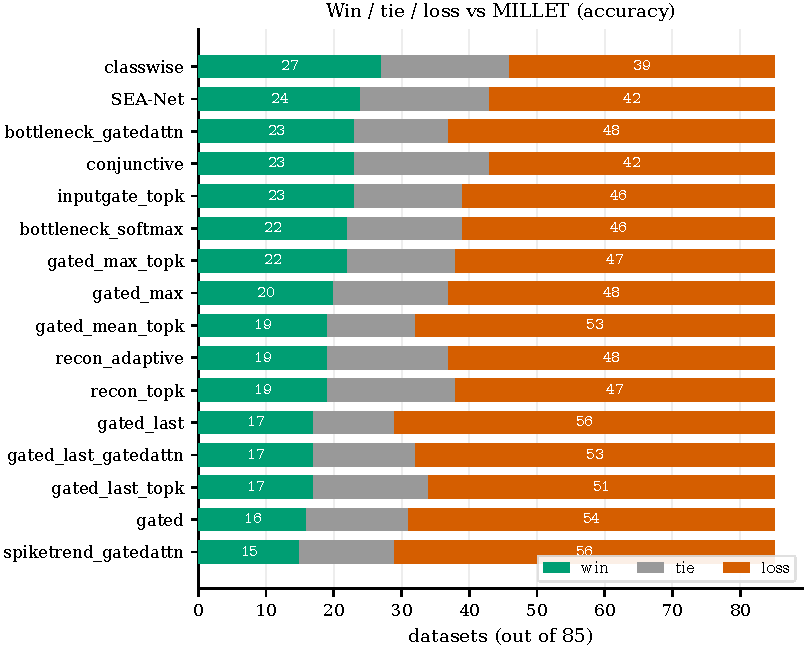
\includegraphics[width=0.68\linewidth]{results/paper_figures/01_main_figures/fig5_win_tie_loss_accuracy}
  \caption{How often each model evaluated on the complete archive beats the published \millet{} results, counted per
  dataset over the 84 datasets both report. A difference below 0.005 counts as a tie, since that is
  below what these test sets can resolve. Rank prefixes use competition ranking, so models with an
  equal number of wins share a rank number and are marked with ``='' -- the two leading models are
  tied at 26 wins each. Read together with the mean accuracy in \Cref{tab:ucr_accuracy}: the mean
  says how large the gap is, this figure says how often it goes each way.}
  \label{fig:acc_diff}
\end{figure}

The shape of \Cref{fig:acc_diff} is its message: wins and losses are spread across the whole
archive rather than concentrated in a few datasets, so the near-balanced aggregate record of
\Cref{tab:ucr_accuracy} is real rather than an artefact of how ties are counted.

\paragraph{Accuracy against series length.}
Does the capped dilation hurt on long series? Checked on \mbot{} over all 128 \ucr{} datasets and
averaged over its 3 seeds, the correlation between accuracy and series length is $-0.34$; splitting
the archive at the median length (344 time steps), the shorter half averages 0.857 accuracy and the
longer half 0.755, a gap of about 10 points. This is consistent with the mechanism: $\delta_{\max}$
is 16 in every \seanet{} configuration (\Cref{sec:arch:block}), so the receptive field stops growing
after a fixed reach and later blocks then operate on an increasingly incomplete view. The effect
size is far larger than any seed-to-seed spread measured (\Cref{tab:seeds}), so it is a real
limitation of the design rather than noise, and adapting the cap is listed as future work in
\Cref{sec:future}.
